\section{Tillitsregionmetoder}
\label{sec:trust_region_methods}

Tillitsregionmetoder er en klasse av optimeringsalgoritmer som skiller seg fundamentalt fra linjesøkmetoder i sin tilnærming. Mens linjesøkmetoder først velger en søkeretning og deretter bestemmer en passende steglengde, definerer tillitsregionmetoder et område rundt det nåværende punktet hvor vi stoler på at modellen av funksjonen er nøyaktig, og bestemmer både retning og steglengde samtidig.

\subsection{Grunnleggende prinsipper og formulering}
\label{subsec:trust_region_principles}

I tillitsregionmetoder konstruerer vi en modell \(m_k\) av objektfunksjonen \(f\) rundt den nåværende iterasjonen \(\symbf{x}_k\). Denne modellen er vanligvis en kvadratisk approksimasjon:

\begin{equation}
	m_k(\symbf{p}) = f(\symbf{x}_k) + \nabla f(\symbf{x}_k)^T\symbf{p} + \frac{1}{2}\symbf{p}^T\symbf{B}_k\symbf{p}
\end{equation}

hvor \(\symbf{B}_k\) er en symmetrisk matrise som approksimerer Hessianen \(\nabla^2 f(\symbf{x}_k)\), og \(\symbf{p}\) representerer et potensielt steg fra det nåværende punktet.

I hver iterasjon løser vi følgende begrensede optimeringsunderproblem:

\begin{equation}
	\min_{\symbf{p} \in \mathbb{R}^n} m_k(\symbf{p}) \quad \text{slik at} \quad \|\symbf{p}\| \leq \Delta_k
\end{equation}

hvor \(\Delta_k > 0\) er radiusen til tillitsregionen, som definerer området rundt \(\symbf{x}_k\) hvor vi stoler på at modellen er nøyaktig.

\begin{definition}{Tillitsregion}{trust_region}
	En \textbf{tillitsregion} er et område rundt den nåværende iterasjonen \( \symbf{x}_k \) hvor vi antar at den kvadratiske modellen \( m_k(\symbf{p}) \) er en tilstrekkelig representasjon av objektfunksjonen \( f(\symbf{x}) \).
	\[
		\mathcal{D}_k = \{\symbf{x} : \|\symbf{x} - \symbf{x}_k\| \leq \Delta_k\}
	\]
	hvor \( \Delta_k \) er radiusen til tillitsregionen.
\end{definition}

\begin{figure}[H]
	\centering
	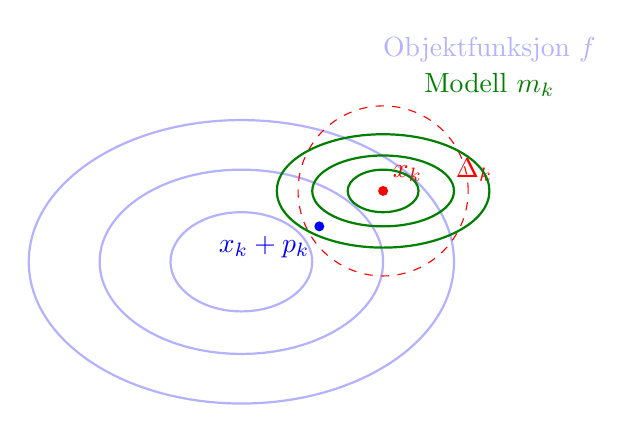
\begin{tikzpicture}[scale=0.9]
		% Konturlinjer for den faktiske funksjonen
		\draw[blue!30, thick] (0,0) ellipse (3 and 2);
		\draw[blue!30, thick] (0,0) ellipse (2 and 1.3);
		\draw[blue!30, thick] (0,0) ellipse (1 and 0.7);

		% Nåværende punkt
		\fill[red] (2,1) circle (2pt) node[above right] {$\symbf{x}_k$};

		% Tillitsregion
		\draw[red, dashed] (2,1) circle (1.2) node[above right, xshift=0.8cm] {$\Delta_k$};

		% Konturlinjer for modellen
		\draw[green!50!black, thick] (2,1) ellipse (1.5 and 0.8);
		\draw[green!50!black, thick] (2,1) ellipse (1 and 0.5);
		\draw[green!50!black, thick] (2,1) ellipse (0.5 and 0.3);

		% Løsningspunkt
		\fill[blue] (1.1,0.5) circle (2pt) node[below left] {$\symbf{x}_k + \symbf{p}_k$};

		% Legende
		\node[blue!30] at (3.5,3) {Objektfunksjon $f$};
		\node[green!50!black] at (3.5,2.5) {Modell $m_k$};
	\end{tikzpicture}
	\caption{Tillitsregionmetode: Den røde sirkelen representerer tillitsregionen med radius $\Delta_k$ rundt det nåværende punktet $\symbf{x}_k$. De blå konturlinjene viser den faktiske objektfunksjonen, mens de grønne konturlinjene viser modellen. Den optimale løsningen av underproblemet gir neste punkt $\symbf{x}_k + \symbf{p}_k$.}
	\label{fig:trust_region}
\end{figure}

\begin{figure}[H]
	\centering
	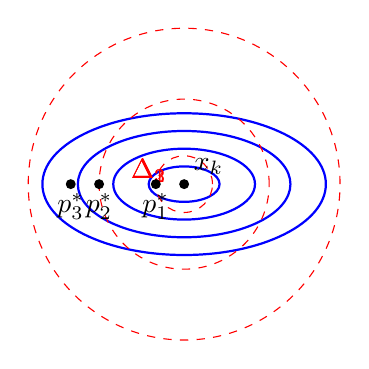
\begin{tikzpicture}[scale=0.9]
		% Konturlinjer for modellen
		\draw[blue, thick] (0,0) ellipse (2 and 1);
		\draw[blue, thick] (0,0) ellipse (1.5 and 0.75);
		\draw[blue, thick] (0,0) ellipse (1 and 0.5);
		\draw[blue, thick] (0,0) ellipse (0.5 and 0.25);

		% Forskjellige tillitsregioner
		\draw[red, dashed] (0,0) circle (0.4) node[above left, xshift=-0.1cm, yshift=-0.1cm] {\( \Delta_1 \)};
		\draw[red, dashed] (0,0) circle (1.2) node[above left, xshift=-0.1cm, yshift=-0.1cm] {\( \Delta_2 \)};
		\draw[red, dashed] (0,0) circle (2.2) node[above left, xshift=-0.1cm, yshift=-0.1cm] {\( \Delta_3 \)};

		% Nåværende punkt
		\fill (0,0) circle (2pt) node[above right] {\( \symbf{x}_k \)};

		% Løsningspunkter
		\fill (-0.4,0) circle (2pt) node[below] {\( \symbf{p}_1^\ast \)};
		\fill (-1.2,0) circle (2pt) node[below] {\( \symbf{p}_2^\ast \)};
		\fill (-1.6,0) circle (2pt) node[below] {\( \symbf{p}_3^\ast \)};

	\end{tikzpicture}
	\caption{Løsninger av tillitsregion-underproblemet for forskjellige radier \( \Delta_1 \), \( \Delta_2 \), \( \Delta_3 \). For liten radius (\( \Delta_1 \)) ligger løsningen på grensen, for middels radius (\( \Delta_2 \)) også på grensen, mens for stor radius (\( \Delta_3 \)) er løsningen den ubegrensede minimeren.}
	\label{fig:trust_region_solutions}
\end{figure}

\subsection{Tillitsregionalgoritme}
\label{subsec:trust_region_algorithm}

Nøkkelen i en tillitsregionalgoritme er hvordan man velger tillitsregionens radius \( \Delta_k \) i hver iterasjon. Dette valget er basert på forholdet \( \rho_k \), som måler hvor godt modellen predikerer den faktiske reduksjonen i objektfunksjonen:

\begin{equation}
	\rho_k = \frac{\text{faktisk reduksjon}}{\text{predikert reduksjon}} = \frac{f(\symbf{x}_k) - f(\symbf{x}_k + \symbf{p}_k)}{m_k(\symbf{0}) - m_k(\symbf{p}_k)}
\end{equation}

Basert på dette forholdet oppdaterer vi tillitsregionens radius og bestemmer om steget skal aksepteres:

\begin{algorithm}[H]
	\SetAlgoLined
	\KwIn{Startpunkt \( \symbf{x}_0 \), initial tillitsregionsradius \( \Delta_0 > 0 \), parametere \( 0 < \eta_1 < \eta_2 < 1 \), \( 0 < \gamma_1 < 1 < \gamma_2 \)}
	\KwOut{Løsning \( \symbf{x}^\ast \)}
	\For{\( k = 0, 1, 2, \dots \)}{
		Løs underproblemet for å finne et steg \( \symbf{p}_k \)\;
		Beregn forholdet:
		\[
			\rho_k = \frac{f(\symbf{x}_k) - f(\symbf{x}_k + \symbf{p}_k)}{m_k(\symbf{0}) - m_k(\symbf{p}_k)}
		\]\;
		Oppdater punktet:
		\[
			\symbf{x}_{k+1} = \begin{cases}
				\symbf{x}_k + \symbf{p}_k, & \rho_k \geq \eta_1, \\[6pt]
				\symbf{x}_k,               & \rho_k < \eta_1.
			\end{cases}
		\]\;
		Oppdater tillitsregionen:
		\[
			\Delta_{k+1} = \begin{cases}
				\gamma_1 \Delta_k, & \rho_k < \eta_1 \quad \text{(dårlig prediksjon)}                 \\
				\Delta_k,          & \eta_1 \leq \rho_k < \eta_2 \quad \text{(akseptabel prediksjon)} \\
				\gamma_2 \Delta_k, & \rho_k \geq \eta_2 \quad \text{(utmerket prediksjon)}
			\end{cases}
		\]
	}
	\caption{Tillitsregionalgoritme}
	\label{alg:trust_region_2}
\end{algorithm}
